\documentclass[t,ignorenonframetext]{beamer}
%\usepackage{beamerthemeJuanLesPins}%
%\usepackage{beamercolorthemecougar} 
%\usepackage{beamerinnerthemecircles} 
\mode<presentation>
{
  \usetheme{Darmstadt}
  \usecolortheme{rose}
  \usefonttheme{default}
}

%\usefonttheme{structuresmallcapsserif}
\usepackage{enumerate,graphicx,verbatim,url}
\usepackage{fancyvrb}
\usepackage{graphicx}
\usepackage{algorithmic}


\newcommand\Red[1]{\textcolor{red}{#1}}

\usepackage{tikz}
\usetikzlibrary{arrows,decorations.pathmorphing,fit,positioning}

% The line below is what I talked about that makes all
% items in a list into overlays
%\beamerdefaultoverlayspecification{<+->}

\newcommand{\tc}[1]{$\backslash$\texttt{#1}}

\title{TITLE}
\author{David van Erkelens, Elise Koster \& Sharon Gieske}
\begin{document}
\frame{
\maketitle
}
\frame{
\tableofcontents
}

\section[Introduction]{Introduction}

\subsection{Motivation}
\begin{frame}
\frametitle{Motivation}~\\



\end{frame}

\subsection{Research Question}
\begin{frame}
\frametitle{Research Question}
 ~\\ ~\\ ~\\


\end{frame}

\begin{frame}~\\

\frametitle{Subquestions}

\end{frame}



\subsection{Related research}~\\


\begin{frame}
\frametitle{Related research}
~\\

\end{frame}


\section[Approach]{Approach}
\subsection{Methods}

\begin{frame}
\frametitle{Plate Diagram}~\\
\begin{figure}[htp]
  \centering
  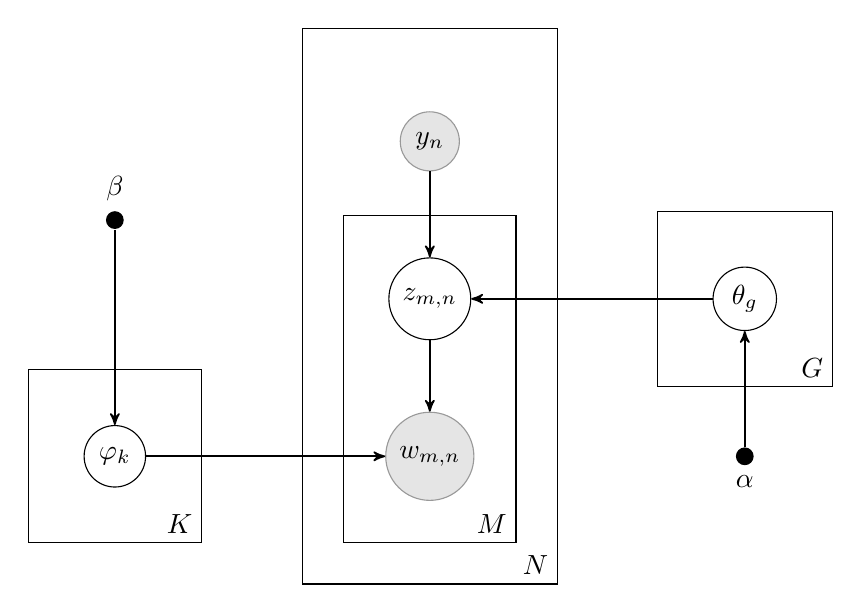
\begin{tikzpicture}
    [
      observed/.style={minimum size=15pt,circle,draw=gray!80,fill=gray!20},
      unobserved/.style={minimum size=15pt,circle,draw},
      hyper/.style={minimum size=1pt,circle,fill=black},
      post/.style={->,>=stealth',semithick},
    ]

    \node (w-j) [observed] at (0,0) {$w_{m,n}$};
    
    \node (z-j) [unobserved] at (0,2) {$z_{m,n}$};

    \node (y) [observed] at (0,4) {$y_n$};
    
    \node (z-prior) [unobserved] at (4,2) {$\theta_g$};
    
    \node (w-prior) [unobserved] at (-4,0) {$\varphi_k$};
    
    \node (z-hyper) [label=below:$\alpha$] at (4,0) {};
    
    \filldraw [black] (4,0) circle (3pt);
    
    \node (w-hyper) [label=above:$\beta$] at (-4,3) {};
    
    \filldraw [black] (-4,3) circle (3pt);
    
    \path
    (z-j) edge [post] (w-j)
    
    (z-hyper) edge [post] (z-prior)
    (z-prior) edge [post] (z-j)
    (y) edge [post] (z-j)


    (w-hyper) edge [post] (w-prior)
    
    (w-prior) edge [post] (w-j)
    ;

    \node [draw,fit=(w-j) (y), inner sep=30pt] (plate-context) {};
    \node [above left] at (plate-context.south east) {$N$};
    \node [draw, fit=(w-prior), inner sep=20pt] (plate-prior) {};
    \node [above left] at (plate-prior.south east) {$K$};
    \node [draw,fit=(w-j) (z-j), inner sep=15pt] (plate-token) {};
    \node [above left] at (plate-token.south east) {$M$};
    \node [draw, fit=(z-prior), inner sep=20pt] (plate-z-prior) {};
    \node [above left] at (plate-z-prior.south east) {$G$};

  \end{tikzpicture}
  \caption{Graphical model}
  \label{fig:graphical-model}
\end{figure}


\end{frame}



\section[Results]{Results}
\begin{frame}
\end{frame}

\section{Conclusion}
\subsection{Conclusion}
\begin{frame}
\frametitle{Conclusions}~\\~\\
\begin{itemize}
\setlength{\itemsep}{10pt}\setlength{\itemsep}{5pt}
\item Can be used to identify type of flights and duration
\item However, no detailed information of flights
\item Logbook records flights (and crashes)
\item Logbook modifications inconsistent with other files
\end{itemize}
\end{frame}

\section[Questions]{Questions}
\begin{frame}
~ \\~ \\~ \\ ~ \\~ \\
\begin{center}\Huge Questions? \end{center} 
\end{frame}

\begin{frame}[allowframebreaks]
        \frametitle{References}
        \bibliographystyle{unsrt}
        \bibliography{../papers/bibliography.bib}
\end{frame}


\end{document}